\documentclass[10pt]{article}
\usepackage{cite}
\usepackage{amsmath}
\usepackage{graphicx}
\usepackage{lipsum}
\usepackage{tikz}
\usepackage{url}
\usepackage{braket}
\usepackage{listings}

\lstset{ %
language=C++,                % choose the language of the code
basicstyle=\scriptsize\ttfamily,       % the size of the fonts that are used for the code
numbers=left,                   % where to put the line-numbers
numberstyle=\footnotesize,      % the size of the fonts that are used for the line-numbers
stepnumber=1,                   % the step between two line-numbers. If it is 1 each line will be numbered
numbersep=5pt,                  % how far the line-numbers are from the code
backgroundcolor=\color{white},  % choose the background color. You must add \usepackage{color}
showspaces=false,               % show spaces adding particular underscores
showstringspaces=false,         % underline spaces within strings
showtabs=false,                 % show tabs within strings adding particular underscores
frame=single,           % adds a frame around the code
tabsize=2,          % sets default tabsize to 2 spaces
captionpos=b,           % sets the caption-position to bottom
breaklines=true,        % sets automatic line breaking
breakatwhitespace=false,    % sets if automatic breaks should only happen at whitespace
escapeinside={\%*}{*)}          % if you want to add a comment within your code
}
\begin{document}
\title{A Secure Set Intersection Protocol using Hamming Distance as a Comparator.}
\author{Dr. Amar Rasheed\\ Armstrong State University\\amar.rasheed@armstrong.edu \and Abrahim Ladha\\ Georgia Institute of Technology\\ abrahimladha@protonmail.ch}
\maketitle


\newpage

\section{Introduction}
We propose a method of securely computing set intersections among parties using a hamming distance protocols as a comparator function. 
\section{Background}

What exactly is cryptography? Cryptography is the practice and study of secure communications in the presence of adversaries. It is using Mathematics to secure information. Cryptography is very new and yet very old. Julius Caesar used to encrypt his messages he deemed of military significance using the \textit{Caesar Cipher}, which shifted every letter over by three. The field in which Dr. Rasheed and I studied is called \textit{Secure Mulitparty Computation}. In a given system of $n$ players, each player $P_i$ has a secret input $x_i$. The players want to compute some $f(x_1,x_2,...,x_n)$ while revealing no information about their inputs. A real world example would be if you have three co-workers, and they want to find out who has the highest salary without revealing their salaries to each other. This means we have $n=3$ players, and $f(x_1,x_2,x_3) = max(x_1,x_2,x_3)$. A good MPC protocol satisfies two properties:
\begin{enumerate}
\item Input Privacy - No information about the players inputs should be able to be inferred during the execution of the protocol. The only information that should be inferred is whatever could have been seen by seeing the output of the function alone.
\item Correctness - No player or players who may deviate from the protocol should be able to force honest parties to output an incorrect result.  
\end{enumerate} 
The problem we are trying to solve in this research is to construct a MPC protocol such that each player $P_i$ has an input $x_i$ that is some finite set. and $f(x_1,x_2,...,x_n) = \bigcap_{i=1}^n x_i$. 

This has direct application. Consider the case where $n$ robots wish to communicate. There are eleven frequency channels on which they may decide to send information. Not every robot can always access every channel, but they need to find out which channels they can communicate on. Each players input would be the set of frequencies that they are eligible to communicate on. In the case that a robot is comprised, no information of the other robots is compromised. Even if $n-1$ robots are compromised, no information is revealed about the $n$th robot.

Hamming Distance is a measurement between two bitstrings. It represents the number of substituitions required to make two numbers identical. For example, if $X = 1001$ and $Y = 1101$, then $d_h(X,Y) = 1$. Not related to this research, hamming distances have a lot of unique properties. They form a metric space on $\{0,1\}^n$ (also known as a hamming space). A hamming space can be represented as a $Q_n$ graph with where the hamming distance between any two elements is the shortest walk between their representative two vertices. They have many applications in coding theory, graph theory, cryptography, and information theory.

Oblivious Transfer (OT) is a protocol type in which a sender transfers one of many pieces of information, but is oblivious as to what piece has been transferred.

Threshold homomorphic cryptosystems are systems that in order to decrypt an encrypted message, require the work of several parties is required. If there are $n$ parties, and atleast $t$ of them must aid in the decryption, then we call this a $(t,n)$-threshold scheme. As a more layman example, consider having $n$ parties, and some $n-1$ degree polynomial $\Sigma_{i=1}^{n-1} a_i x^i$ where $a_i$ is an element of some finite field and $\braket{a_1,a_2,...,a_n}$. is our message to decrypt (our shared secret). We give each player some unique point that is a solution to  our polynomial. Clearly if they work together, by methods of Lagrange interpolation they can solve for the coefficients of our polynomial since they have $n$ points points and the polynomial is defined as having degree $n-1$. However this requires all $n$ parties. Even if $n-1$ parties converse, there will be many possible solutions in our field. In the real numbers, given some polynomial of degree $n-1$, and if you don't have $n$ or more points, then there exist infinite solutions for your coefficients of your polynomial. This can be considered a $(n,n)$-threshold scheme, and its called Shamir's Secret sharing scheme.\cite{shamir}
\section{Proposal}
We propose a different solution than in \cite{polynomial}. Given $n$ sets, $x_1,...,x_n$, we compute the intersections of two sets at a time. We compare each element of one set to every element of the other set. If the hamming distance of two elements compared is zero, this implies that they are identical, so they are added to a new temporary set. This temporary set is is then added to the sets to compute the intersection of. If is it the case that some $x_i \cap x_j = \emptyset$ for $i  < j$, then we simply take $x_i$ as it has higher precedence. For the secure hamming distance method, we borrow two protocols from \cite{shade}. known as the basic scheme and the fully secure scheme. They are both secure against different types of adversaries. The basic scheme is secure against semi-honest (passive) adversaries. This means we can assume adversaries cooperate to gather information and do not deviate from the protocol specification. The fully secure scheme is secure against malicious (active) adversaries. In this case they may deviate from the protocol specification and attempt to cheat, as the design of the protocol ensures its a futile endeavor. 


\section{Results}
Due to some issues, The fully secure scheme does not run with out running out of memory. This will continue to be worked on as time progresses. The basic scheme is fully implemented and we have recorded and presented some information based off its efficiency

%add hamming distance vs time
\begin{figure}[ht!]
\centering
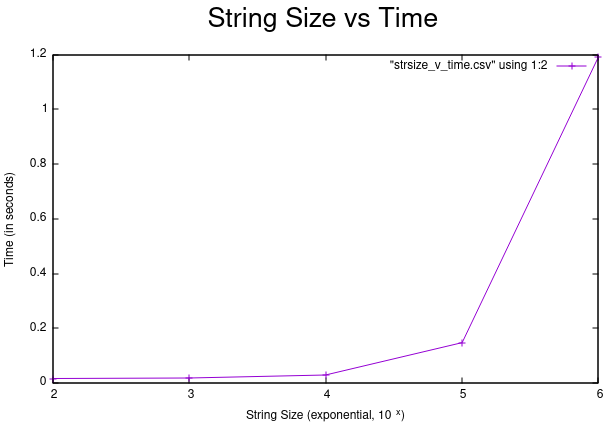
\includegraphics[scale=0.64]{h1} 
\caption{Time taken based on String length. x-scale is exponential to demonstrate that this is infact $O(n)$ and not $O(1)$.}
\end{figure}

\begin{figure}[ht!]
\centering
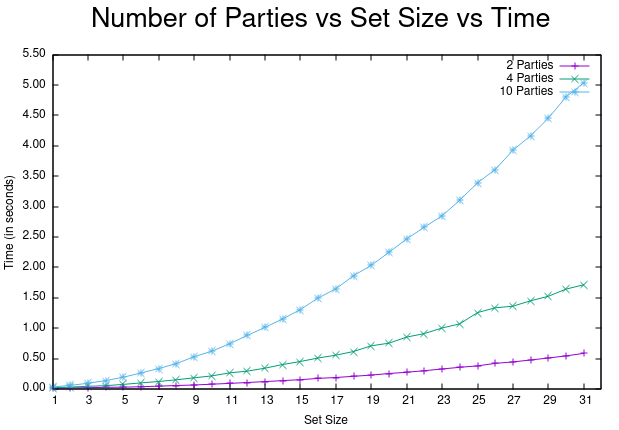
\includegraphics[scale=0.64]{g6} 
\caption{Time in seconds it takes to compute intersection of sets of different sizes. Shown here for 2, 4, and 10 parties}
\end{figure}

Since It takes $O(n)$ time to process a string, and to process sets is a simple combinatorial algorithm running in $O(n\log n)$, the time for this algorithm to run in $O(n^2 \log n^2)$



%add hamming distance vs throughput
%add some random observations about throughput

\section{Appendices}
Here we present the actual code. Please keep in mind files for the fully secure scheme are not implemented correctly but are presented for completion's sake.\\
basic.h
\lstinputlisting{basic.h}
basic.cpp
\lstinputlisting{basic.cpp}
main.cpp
\lstinputlisting{main.cpp}
elgamal\_v.cpp
\lstinputlisting{elgamal_gmpxx.cpp}
fully\_secure.h
\lstinputlisting{fully_secure.h}
fully\_secure.cpp
\lstinputlisting{fully_secure.cpp}
elgamal.h
\lstinputlisting{elgamal.h}
elgamal.cpp
\lstinputlisting{elgamal.cpp}
crypto.cpp
\lstinputlisting{crypto.cpp}
%main.cpp

%elgamal.cpp
%elgamal.h
%elgamal_prover.cpp
%elgamal_prover.h

%basic.cpp
%basic.h

%fully_secure.h
%fully_secure.cpp
%
\begin{thebibliography}{1}

\bibitem{shade} Julien Bringer, Herve Chabanné, Alain Patey {\em SHADE: Secure HAmming DistancE computation from oblivious transfer.} 2012.
%shade paper

\bibitem{shamir} Adi Shamir {\em How to Share a Secret.} 1979.
%shamirs scheme

\bibitem{polynomial} Benny Pinkas, Thomas Schneider, Michael Zohner {\em Faster Private Set Intersection based on OT Extension} 2014.

\bibitem{bitstrings} Mehmet S. Kiraz,, Berry Schoenmakers, José Villegas {\em Efficient Commited Oblivious Transfer of Bit Strings.} 2007.

\end{thebibliography}
\end{document}